\documentclass[14pt]{extreport}

% Основные пакеты
\usepackage[english, russian]{babel}    % Поддержка русского и английского языков
\usepackage{graphicx}                   % Для вставки изображений
\usepackage{import}                     % Для продвинутого импорта (например, pdf_tex из Inkscape)
\usepackage{subcaption}                 % Для создания подписей к фигурам
\usepackage{float}                      % Для улучшенного позиционирования фигур
\usepackage{geometry}                   % Для управления отступами на странице
\usepackage{amsmath}                    % Для расширенной поддержки математики
\usepackage{amsfonts}                   % Математические шрифты
\usepackage{amssymb}                    % Математические символы
\usepackage{tabu}                       % Улучшенные таблицы
\usepackage{booktabs}                   % Профессиональные таблицы с вертикальными разделителями
\usepackage[dvipsnames]{xcolor}         % Расширенная поддержка цветов
\usepackage{longtable}                  % Для таблиц, занимающих несколько страниц
\usepackage{makecell}                   % Для улучшенного форматирования ячеек таблиц
\usepackage{multirow}                   % Для объединения строк в таблицах
\usepackage{tabularray}                 % Для современных таблиц
\usepackage{varwidth}                   % Для переменной ширины блоков
\usepackage{hyperref}                   % Для гиперссылок
\usepackage{verbatim}                   % Для вставки кода
\usepackage{listings}                   % Для оформления листингов кода
\usepackage{amsmath}
% Настройка графики
\graphicspath{ {./images/} }            % Путь к папке с изображениями

% Настройка отступов на странице
\geometry{left=2cm, right=2cm, bottom=2cm, top=2cm}

% Настройка гиперссылок
\hypersetup{
	linkcolor=blue,                     % Цвет ссылок
	filecolor=magenta,                  % Цвет ссылок на файлы
	urlcolor=cyan                       % Цвет URL-адресов
}

\definecolor{codegreen}{rgb}{0,0.6,0}  % Цвет для комментариев
\definecolor{codegray}{rgb}{0.5,0.5,0.5}  % Цвет для номеров строк
\definecolor{codepurple}{rgb}{0.58,0,0.82}  % Цвет для строк
\definecolor{backcolour}{rgb}{0.95,0.95,0.92}  % Цвет фона

% Определим стиль для выделения переменных
\lstdefinestyle{codestyle}{
	backgroundcolor=\color{backcolour},  % Цвет фона
	commentstyle=\color{codegreen}\itshape,  % Стиль для комментариев
	keywordstyle=\color{magenta}\bfseries,  % Стиль для ключевых слов
	numberstyle=\tiny\color{codegray},  % Стиль для номеров строк
	stringstyle=\color{codepurple},  % Стиль для строк
	identifierstyle=\color{black},  % Стиль для переменных (выделим их синим)
	basicstyle=\ttfamily\footnotesize,  % Размер шрифта для кода
	breakatwhitespace=false,  % Не разрывать строки в пробелах
	breaklines=true,  % Разбивать длинные строки
	captionpos=b,  % Позиция заголовка (внизу)
	keepspaces=true,  % Сохранять пробелы
	numbers=left,  % Позиция номеров строк
	numbersep=10pt,  % Расстояние между кодом и номерами строк
	showspaces=false,  % Не показывать пробелы
	showstringspaces=false,  % Не показывать пробелы в строках
	showtabs=false,  % Не показывать табуляции
	tabsize=4,  % Размер табуляции
	frame=single,  % Добавить рамку вокруг кода
	rulecolor=\color{black},  % Цвет рамки
	backgroundcolor=\color{backcolour},  % Цвет фона рамки
	xleftmargin=15pt,  % Отступ слева
	xrightmargin=15pt,  % Отступ справа
}


\lstset{style=codestyle}
\lstset{extendedchars=\true}
\graphicspath{{../images/}}

\begin{document}
	
	\begin{titlepage}
		\centering
		\vspace*{1cm}
		
		{\large Министерство науки и высшего образования Российской Федерации}\\
		{\large ФЕДЕРАЛЬНОЕ ГОСУДАРСТВЕННОЕ АВТОНОМНОЕ ОБРАЗОВАТЕЛЬНОЕ УЧРЕЖДЕНИЕ ВЫСШЕГО ОБРАЗОВАНИЯ «НАЦИОНАЛЬНЫЙ ИССЛЕДОВАТЕЛЬСКИЙ УНИВЕРСИТЕТ ИТМО»}\\
		{\large (УНИВЕРСИТЕТ ИТМО)}\\
		
		\vspace{1cm}
		
		\textbf{{\Huge ОТЧЕТ}\\
			{\Huge ПО ЛАБОРАТОРНОЙ РАБОТЕ №4}}\\
		
		\vspace{1cm}
		
		{\LARGE По дисциплине\\
			\(\lll\) Математическая Статистика \(\ggg\) }\\
			Вариант 2
		
		\vspace{2cm}
		
		{\Large Студенты:}\\
		Охрименко Eва\\
		Даниил Буцкий
		
		
		\vspace{2cm}
		
		{\Large Проверил:}\\
		Шкваренко Андрей Алексеевич\\
		
		\vspace{2cm}
		
		{\large г. Санкт-Петербург}\\
		{\large 2025}
		
	\end{titlepage}
	\tableofcontents  % Оглавление
	\newpage

	
	
	\section{Вопрос}
	
	
	В этом задании нужно оценить однородность количества мужчин и жещин в эксперименте. Также нужно оценить этническую принадлежность. Вот код, который считает данные полов и данные этнических принадлежностей из файла:
	
	
	\begin{lstlisting}[language=python, caption={Счет данных по выборкам}]
f = open('exams_dataset.csv')

maleCount = femaleCount = 0
countA = countB = countC = countD = countE = 0

for line in f:
	
	items = line.strip().replace('"', '').split(',')
	
	gender = items[0]
	etnic = items[1]
	
	if gender == 'male':
		maleCount += 1
	elif gender == 'female':
		femaleCount += 1
	
	if etnic[-1] == 'A':
		countA += 1
	elif etnic[-1] == 'B':
		countB += 1
	elif etnic[-1] == 'C':
		countC += 1
	elif etnic[-1] == 'D':
		countD += 1
	elif etnic[-1] == 'E':
		countE += 1


genderArray = list()
etnicArray = list()

genderArray += [maleCount, femaleCount]
etnicArray += [countA, countB,  countC,  countD, countE]
\end{lstlisting}
	
	
	У нас получилось \texttt{506} мужчин и \texttt{494} женщин. Также у нас получился такой массив по этническим группам: \texttt{[77, 204, 324, 261, 134]}. Можно заметить, что массив с полами примерно однороден, а с этническими группами менее однороден.
	
	\subsection{Реализация методов}	
	
	Для этого задания мы напишем 2 статистических метода на питоне. Метод \texttt{хи-квадрат} и метод вычисляющдий \texttt{критерий Когломорова-Смирнова}
	
	Итак, критерий \texttt{хи-квадрат} вычисляется по формуле:
	
	\[
		\chi^2 = \sum_{i=1}^{n} \frac{(O_i - E_i)^2}{E_i}
	\]
	
	где:
	\begin{itemize}
		\item $O_i$ --- наблюдаемые значения (элементы массива \texttt{array})
		\item $E_i = \frac{\sum_{j=1}^{n} O_j}{n}$ --- ожидаемое значение для равномерного распределения
		\item $n$ --- количество элементов в массиве (\texttt{ln = len(array)})
	\end{itemize}
	
	А \texttt{критерий Когломорова-Смирнова} вычисляется так:
	
	\[
		D_n = \sup_x |F_n(x) - F(x)|
	\] 
	
	где:
	\begin{itemize}
		\item $F_n(x)$ --- эмпирическая функция распределения:
		\[
			F_n(x) = \frac{\text{количество элементов} \leq x}{n} = \frac{i}{n} \quad \text{для} \quad x \in [x_{(i)}, x_{(i+1)})
		\] 
		
		\item $F(x)$ --- теоретическая функция равномерного распределения:
		\[
			F(x) = \frac{x}{\max(\text{array})} \quad \text{для} \quad x \in [0, \max(\text{array})]
		\] 
		
		\item $\sup_x$ --- супремум (максимальное отклонение)
	\end{itemize}
	
	Вот реализация кодом:
	
	\begin{lstlisting}[language=python, caption=Расчет хи-квадрат]
def hiQuad(array):
	
	sm = sum(array)
	ln = len(array)
	expected = sm / ln
	
	hiQuad = sum((i - expected)**2 / expected for i in array)   
	
	return round(hiQuad, 4)
\end{lstlisting}
	
	\begin{lstlisting}[language=python, caption=Расчет критерия Когломорова-Смирнова]
def kolmogorovSmirnov(array):
	
	ln = len(array)
	sortArray = np.sort(array)
	
	y = np.arange(1, ln+1) / ln
	teoria = sortArray / np.max(sortArray)
	kriteriy = np.max(np.abs(y - teoria))
	
	return round(kriteriy, 4)
\end{lstlisting}
	
	\subsection{Применение методов к выборкам}
	
	Применяем методы:
	
	\begin{lstlisting}[language=python, caption=Применение метода к гендерам]
result = hiQuad(genderArray)
print(result)

Output >>> 0.144
\end{lstlisting}
	
	
	\begin{lstlisting}[language=python, caption=Применение метода к этникам]
result = kolmogorovSmirnov(etnicArray)
print(result)

Output >>> 0.0377
\end{lstlisting}
	
	\subsection{Оценка и вывод}
	
	
	Для начала сформулируем гипотезы для полов:
	
	\begin{itemize}
		\item \texttt{Нулевая гипотеза:} Распределение полов равномерное (50 на 50)
		\item \texttt{Альтернативная гипотеза:} Распределение полов неравномерное
	\end{itemize}

	Теперь посчитаем критическое значение хи квадрат по таблице из интернета
	
	\begin{figure}[H]
		\centering
		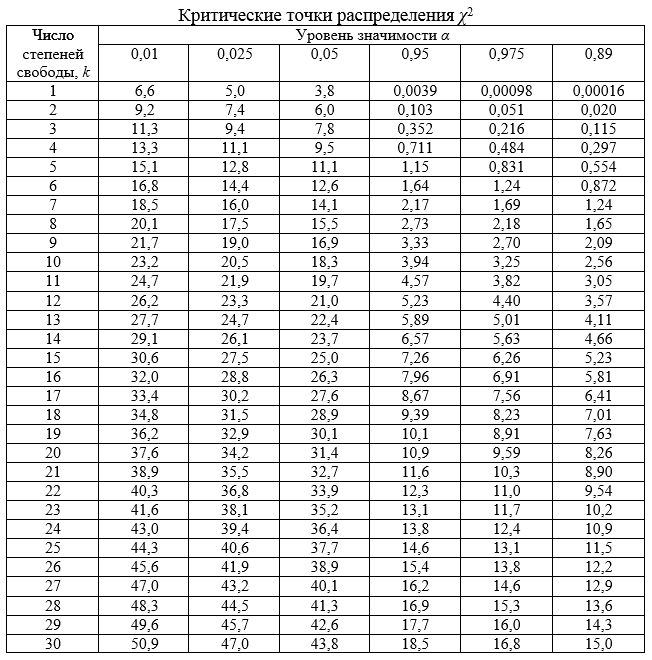
\includegraphics[width=1\textwidth]{table.png}
		\caption{Таблица}
		\label{fig:lines}
	\end{figure}
	
	Нам нужно взять $k = 1$, так как оно считается по формуле $k = iterations - 1$ (посчитали по туториалу)и возьмем $\alpha = 0.05$ - средний уровень значимости
	
	Тогда наше критическое значение $\chi_{crit}^2 = 3.8$. Так как $\chi_{crit}^2 > \chi^2$, то вывод таков: \texttt{распредедление полов равномерное}.
	\\
	\\
	\\
	\\
	
	Теперь сформулируем гипотезы для этнических принадлежностей:
	
	\begin{itemize}
		\item \texttt{Нулевая гипотеза:} Распределение этник равномерное 
		\item \texttt{Альтернативная гипотеза:} Распределение этник неравномерное
	\end{itemize}
	
	Для $\alpha = 0.0377$ и $n=1000$:
	$$
	D_{\text{крит}} = \frac{c(\alpha)}{\sqrt{n}} \approx \frac{1.47}{31.623} \approx 0.0465
	$$
	где $c(0.0377) \approx 1.47$.
	
	Так как $D_n = 0.123 > D_{\text{крит}} = 0.0465$, гипотеза $H_0$ о равномерном распределении не работает. Распределение неравномерно.
	
	
	\section{Вопрос}
	
	В этом задании нам нужно проверить гипотезу на однородность результатов по математике и письменной части. Создадим массив \texttt{[0] * 101} куда будем записывать количество сдавших экзамен на i-тый балл, где i - индекс массива. Вот код:
	
	
	\begin{lstlisting}[language=python, caption={Счет выборок}]
f = open('exams_dataset.csv')
	
resultMath = [0] * 101
resultWrite = [0] * 101

continueCount = 0
	
	for line in f:
		
		continueCount += 1
		if continueCount == 1:
			continue
		
		items = line.strip().replace('"', '').split(',')
		
		resultMath[int(items[-3])] += 1
		resultWrite[int(items[-1])] += 1
\end{lstlisting}
	
	Теперь напишем статистические тесты. Возьмем уже готовые тесты хи-квадрат и Когломорова-Смирнова. Проведем хи-квадрат для выборки \texttt{resultMath}:
	
	\begin{lstlisting}[language=python, caption=$\chi^2$-тест]
obs = [x for x in resultMath if x > 0]
exp = [sum(obs)/len(obs)] * len(obs)
		
_, p = chisquare(obs, exp)
print("Неравномерное" if p < 0.05 else "Равномерное")

Output >>> Неравномерное
\end{lstlisting}
	
	И действительно, данные неоднородны. Это можно заметить(даже без точных тестов) по распределению баллов:
	
	\begin{figure}[H]
		\centering
		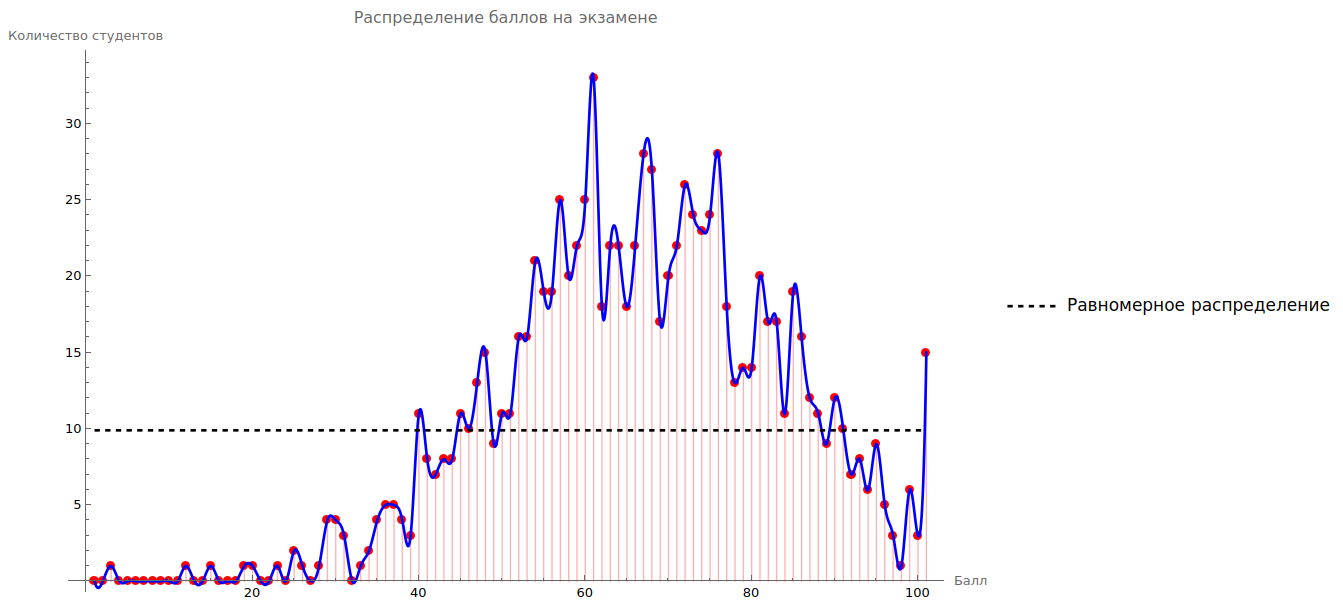
\includegraphics[width=1\textwidth]{resultMath.png}
		\label{fig:lines}
	\end{figure} 
	
	
	Теперь проведем встроенный тест Когломорова-Смирнова на выборке с результатами по письму.
	
	\begin{lstlisting}[language=python, caption=K-S тест]
obs = [x for x in resultWrite if x > 0]
exp = [sum(obs)/len(obs)] * len(obs)

ks_stat, ks_p = stats.kstest(obs, 'uniform', args=(min(obs), max(obs) - min(obs)))
print("Неравномерное" if ks_p < 0.05 else "Равномерное")
	
Output >>> Неравномерное
\end{lstlisting}

Также посмотрим на распределение баллов и убедимся в правильности теста:

	\begin{figure}[H]
		\centering
		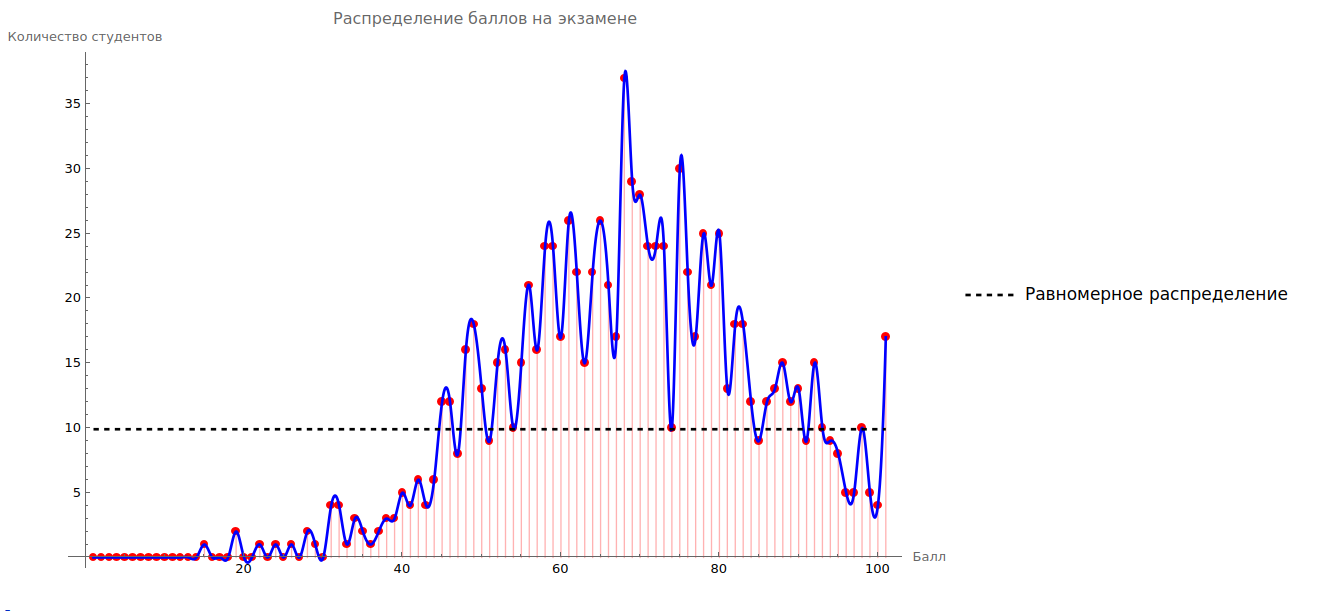
\includegraphics[width=1\textwidth]{resultWrite.png}
		\label{fig:lines}
	\end{figure} 


\section{Вопрос}

Верно ли, что прошедшие подготовительные курсы студенты лучше сдали экзамены?

\subsection{Формализация гипотез:}


$H_0$: Нет различий в средних баллах по математике между теми, кто посещал подготовительные курсы, и теми, кто их не посещал.


$H_1$: Те, кто прошёл подготовительные курсы, лучше сдали математику (средний балл выше).

\subsection{Проверка гипотезы}

\textbf{Шаг 1. Объединение и ранжирование}

\begin{itemize}
    \item Объединяем все значения из обеих групп в один массив.
    \item Сортируем этот массив по возрастанию.
    \item Каждому элементу присваиваем ранг: самое маленькое значение - ранг 1, следующее - 2 и т.д.
    \item Если встречаются одинаковые значения (тай), им присваивается средний ранг для их позиций.
\end{itemize}

\textbf{Шаг 2. Сумма рангов по группам}

Считаем сумму рангов для первой группы ($R_1$) и второй группы ($R_2$).

\textbf{Шаг 3. Вычисление U-статистики}

Для каждой группы считается своё значение $U$:

\[
U_1 = R_1 - \frac{n_1(n_1+1)}{2}
\]
\[
U_2 = R_2 - \frac{n_2(n_2+1)}{2}
\]

$U_1$ - число случаев, когда значение из первой группы больше значения из второй.

$U_2$ - наоборот.


Обычно для теста берут минимальное из этих двух значений.

\textbf{Шаг 4. Подсчет вероятности (p-value)}

\[
\mu_U = \frac{n_1 n_2}{2}
\]
\[
\sigma_U = \sqrt{ \frac{n_1 n_2 (n_1 + n_2 + 1)}{12} }
\]
\[
Z = \frac{U - \mu_U}{\sigma_U}
\]

$Z$ - стандартная нормальная статистика.

$p$-value - вероятность получить $|Z|$ или большее значение по стандартному нормальному распределению (двусторонний тест).

Я решил провести тесты с помощью U-критерия Манна-Уитни, потому что распределение ненормальное. Один тест я буду проводить с помощью теста из библиотеки, а другой написанный вручную.

Вот код, который делает это:

\begin{lstlisting}[language=python, caption=K-S тест]
import pandas as pd
import matplotlib.pyplot as plt
import seaborn as sns
from scipy.stats import mannwhitneyu, norm
import numpy as np
from scipy.stats import norm

# Загрузка данных
df = pd.read_csv('exams_dataset.csv')

# Создаем суммарный балл по трём экзаменам
df['total_score'] = df['math score'] + df['reading score'] + df['writing score']

# Разделение на группы
completed = df[df['test preparation course'] == 'completed']['total_score']
none = df[df['test preparation course'] == 'none']['total_score']

# --- Тест 1: Манн–Уитни с библиотекой ---
stat, p_lib = mannwhitneyu(completed, none, alternative='greater')
print(f"Библиотечный Mann-Whitney U test:\nU={stat:.0f}, p={p_lib:.6e}")

# --- Тест 2: Собственная реализация Манн–Уитни U-теста ---
def mannwhitneyu_manual(x, y):
    # Сортируем объединённые значения и присваиваем ранги
    all_values = np.concatenate([x, y])
    ranks = pd.Series(all_values).rank(method='average').values
    # Ранги для первой группы
    ranks_x = ranks[:len(x)]
    # Сумма рангов первой группы
    R1 = ranks_x.sum()
    n1 = len(x)
    n2 = len(y)
    # U-статистика для первой группы
    U1 = R1 - n1 * (n1 + 1) / 2
    # U-статистика для второй группы (по определению)
    U2 = n1 * n2 - U1
    U = min(U1, U2)

    mu_U = n1 * n2 / 2
    sigma_U = np.sqrt(n1 * n2 * (n1 + n2 + 1) / 12)
    z = (U - mu_U) / sigma_U
    # Двусторонний p-value
    p_manual = 2 * norm.cdf(-abs(z))
    return U, p_manual

U_man, p_man = mannwhitneyu_manual(completed, none)
print(f"Ручной Mann-Whitney U test:\nU={U_man:.0f}, p={p_man:.6e}")


# --- Визуализация: только violin plot ---
plt.figure(figsize=(8, 6))
sns.violinplot(x='test preparation course', y='total_score', data=df, inner="quartile", split=True)
plt.title('Плотность распределения суммарных баллов по экзаменам\nв зависимости от прохождения подготовительных курсов')
plt.xlabel('Подготовительные курсы')
plt.ylabel('Суммарный балл')
plt.tight_layout()
plt.show()
\end{lstlisting}

Вывод программы:

\begin{figure}[H]
    \centering
    
\includegraphics[width=1\textwidth]{tex/3_2.png}
\end{figure}

Вывод ручного и автоматического теста отличается, потому что в автоматической функции, выводится значения для первой выборки, а в ручном выводится минимальное значение U между двумя выборками. U1 почти в 2 раза больше, чем U2, что также подтверждает, что в большинстве случаев, луди, прошедшие подготовительные курсы сдают лучше.

Оба теста Манна–Уитни (библиотечный и ручной) показали крайне малое p-value ($p \ll 0.05$), что позволяет с высокой уверенностью утверждать: прошедшие подготовительные курсы сдают экзамены лучше, чем не прошедшие.


Также рассмотрим распределение 2 типов студентов, чтобы наглядно увидеть, что факт прохождения подготовительных курсов, является значимым:

\begin{figure}[H]
    \centering
    
\includegraphics[width=0.7\textwidth]{tex/3_1.png}
\end{figure}


\end{document}